\documentclass{article}
\usepackage{graphicx} % Required for inserting images
\usepackage[T2A]{fontenc}
\usepackage{titlesec}
%\usepackage{verbatim}
\usepackage[left=25mm, right=15mm, top=20mm, bottom=20mm, footskip=10mm]{geometry}
\usepackage{amsmath}
\usepackage{epigraph}
\usepackage{tikz}
\usepackage{latexsym}
%\usepackage{listings}
\frenchspacing 
\newcommand{\path}{\rightsquigarrow}
\titleformat{\section}[hang]{\normalsize\bfseries}{\thesection~}{0pt}{}
\titlespacing{\section}{\parindent}{\baselineskip}{\baselineskip}

\titleformat{\subsection}[hang]{\normalsize}{\thesubsection~}{0pt}{}
\titlespacing{\subsection}{\parindent}{0pt}{0pt}
\parindent=1.25cm 

\title{Тема 3. Обход в глубину. Восстановление пути. Обход графов с неявным списком смежности }
\date{}

\begin{document}

\maketitle

\epigraph{Автор конспекта: Родион Лыков}


\section{Обход в глубину с восстановлением ответа}

Итак, давайте научимся решать такую задачу: найти любой путь из вершины $S$ в вершину $T$. Рассмотрим следующий граф, который мы уже рассматривали на прошлой лекции:

\begin{center}
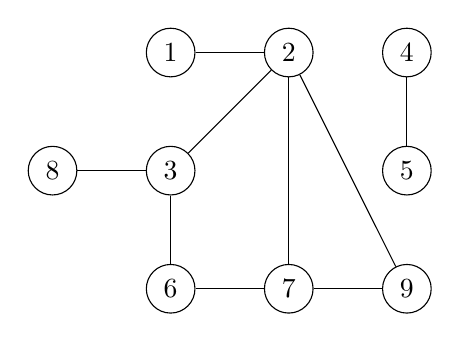
\begin{tikzpicture}[main/.style = {draw, circle},node distance={15mm}] 
\node[main] (1) []{$1$}; 
\node[main] (2) [right of=1] {$2$}; 
\node[main] (3) [below of=1] {$3$};
\node[main] (4) [right of=2] {$4$};
\node[main] (5) [below of=4] {$5$};
\node[main] (6) [below of=3] {$6$};
\node[main] (7) [right of=6] {$7$};
\node[main] (8) [left of=3] {$8$};
\node[main] (9) [right of=7] {$9$};
\draw (1) -- (2);
\draw (2) -- (3);
\draw (4) -- (5);
\draw (8) -- (3);
\draw (3) -- (6);
\draw (7) -- (6);
\draw (7) -- (2);
\draw (7) -- (9);
\draw (2) -- (9);
\end{tikzpicture} 

\end{center}

Найдем любой путь $1 \rightarrow 9$. Давайте запустим обход в глубину и выпишем все вершины на текущем пути:

\begin{tikzpicture}[main/.style = {draw, circle},node distance={15mm}] 
\node[main] (1) [fill=red]{$1$}; 
\node[main] (2) [right of=1] {$2$}; 
\node[main] (3) [below of=1] {$3$};
\node[main] (4) [right of=2] {$4$};
\node[main] (5) [below of=4] {$5$};
\node[main] (6) [below of=3] {$6$};
\node[main] (7) [right of=6] {$7$};
\node[main] (8) [left of=3] {$8$};
\node[main] (9) [right of=7] {$9$};
\draw (1) -- (2);
\draw (2) -- (3);
\draw (4) -- (5);
\draw (8) -- (3);
\draw (3) -- (6);
\draw (7) -- (6);
\draw (7) -- (2);
\draw (7) -- (9);
\draw (2) -- (9);
\node[align = center, below of = 7] {Путь: $[1]$};
\end{tikzpicture} 
\qquad \begin{tikzpicture}[main/.style = {draw, circle},node distance={15mm}] 
\node[main] (1) [fill=green]{$1$}; 
\node[main] (2) [right of=1][fill=red] {$2$}; 
\node[main] (3) [below of=1] {$3$};
\node[main] (4) [right of=2] {$4$};
\node[main] (5) [below of=4] {$5$};
\node[main] (6) [below of=3] {$6$};
\node[main] (7) [right of=6] {$7$};
\node[main] (8) [left of=3] {$8$};
\node[main] (9) [right of=7] {$9$};
\draw (1) -- (2);
\draw (2) -- (3);
\draw (4) -- (5);
\draw (8) -- (3);
\draw (3) -- (6);
\draw (7) -- (6);
\draw (7) -- (2);
\draw (7) -- (9);
\draw (2) -- (9);
\node[align = center, below of = 7] {Путь: $[1,2]$};
\end{tikzpicture} 
\newline \newline \newline
\begin{tikzpicture}[main/.style = {draw, circle},node distance={15mm}] 
\node[main] (1) [fill=green]{$1$}; 
\node[main] (2) [right of=1][fill=green] {$2$}; 
\node[main] (3) [below of=1] {$3$};
\node[main] (4) [right of=2] {$4$};
\node[main] (5) [below of=4] {$5$};
\node[main] (6) [below of=3] {$6$};
\node[main] (7) [right of=6][fill=red] {$7$};
\node[main] (8) [left of=3] {$8$};
\node[main] (9) [right of=7] {$9$};
\draw (1) -- (2);
\draw (2) -- (3);
\draw (4) -- (5);
\draw (8) -- (3);
\draw (3) -- (6);
\draw (7) -- (6);
\draw (7) -- (2);
\draw (7) -- (9);
\draw (2) -- (9);
\node[align = center, below of = 7] {Путь: $[1,2,7]$};
\end{tikzpicture} 
\qquad \begin{tikzpicture}[main/.style = {draw, circle},node distance={15mm}] 
\node[main] (1) [fill=green]{$1$}; 
\node[main] (2) [right of=1][fill=green] {$2$}; 
\node[main] (3) [below of=1] {$3$};
\node[main] (4) [right of=2] {$4$};
\node[main] (5) [below of=4] {$5$};
\node[main] (6) [below of=3][fill=red] {$6$};
\node[main] (7) [right of=6][fill=green] {$7$};
\node[main] (8) [left of=3] {$8$};
\node[main] (9) [right of=7] {$9$};
\draw (1) -- (2);
\draw (2) -- (3);
\draw (4) -- (5);
\draw (8) -- (3);
\draw (3) -- (6);
\draw (7) -- (6);
\draw (7) -- (2);
\draw (7) -- (9);
\draw (2) -- (9);
\node[align = center, below of = 7] {Путь: $[1,2,7,6]$};
\end{tikzpicture} 
\newline \newline \newline
\begin{tikzpicture}[main/.style = {draw, circle},node distance={15mm}] 
\node[main] (1) [fill=green]{$1$}; 
\node[main] (2) [right of=1][fill=green] {$2$}; 
\node[main] (3) [below of=1][fill=red] {$3$};
\node[main] (4) [right of=2] {$4$};
\node[main] (5) [below of=4] {$5$};
\node[main] (6) [below of=3][fill=green] {$6$};
\node[main] (7) [right of=6][fill=green] {$7$};
\node[main] (8) [left of=3] {$8$};
\node[main] (9) [right of=7] {$9$};
\draw (1) -- (2);
\draw (2) -- (3);
\draw (4) -- (5);
\draw (8) -- (3);
\draw (3) -- (6);
\draw (7) -- (6);
\draw (7) -- (2);
\draw (7) -- (9);
\draw (2) -- (9);
\node[align = center, below of = 7] {Путь: $[1,2,7,6,3]$};
\end{tikzpicture} 
\qquad \begin{tikzpicture}[main/.style = {draw, circle},node distance={15mm}] 
\node[main] (1) [fill=green]{$1$}; 
\node[main] (2) [right of=1][fill=green] {$2$}; 
\node[main] (3) [below of=1][fill=green] {$3$};
\node[main] (4) [right of=2] {$4$};
\node[main] (5) [below of=4] {$5$};
\node[main] (6) [below of=3][fill=green] {$6$};
\node[main] (7) [right of=6][fill=green] {$7$};
\node[main] (8) [left of=3][fill=red] {$8$};
\node[main] (9) [right of=7] {$9$};
\draw (1) -- (2);
\draw (2) -- (3);
\draw (4) -- (5);
\draw (8) -- (3);
\draw (3) -- (6);
\draw (7) -- (6);
\draw (7) -- (2);
\draw (7) -- (9);
\draw (2) -- (9);
\node[align = center, below of = 7] {Путь: $[1,2,7,6,3,8]$};
\end{tikzpicture} 
% 1->2->3->6
\newline \newline \newline
\begin{tikzpicture}[main/.style = {draw, circle},node distance={15mm}] 
\node[main] (1) [fill=green]{$1$}; 
\node[main] (2) [right of=1][fill=green] {$2$}; 
\node[main] (3) [below of=1][fill=green] {$3$};
\node[main] (4) [right of=2] {$4$};
\node[main] (5) [below of=4] {$5$};
\node[main] (6) [below of=3][fill=green] {$6$};
\node[main] (7) [right of=6][fill=red] {$7$};
\node[main] (8) [left of=3][fill=green] {$8$};
\node[main] (9) [right of=7] {$9$};
\draw (1) -- (2);
\draw (2) -- (3);
\draw (4) -- (5);
\draw (8) -- (3);
\draw (3) -- (6);
\draw (7) -- (6);
\draw (7) -- (2);
\draw (7) -- (9);
\draw (2) -- (9);
\node[align = center, below of = 7] {Путь: $[1,2,7]$};
\end{tikzpicture} 
\qquad \begin{tikzpicture}[main/.style = {draw, circle},node distance={15mm}] 
\node[main] (1) [fill=green]{$1$}; 
\node[main] (2) [right of=1][fill=green] {$2$}; 
\node[main] (3) [below of=1][fill=green] {$3$};
\node[main] (4) [right of=2] {$4$};
\node[main] (5) [below of=4] {$5$};
\node[main] (6) [below of=3][fill=green] {$6$};
\node[main] (7) [right of=6][fill=green] {$7$};
\node[main] (8) [left of=3][fill=green] {$8$};
\node[main] (9) [right of=7][fill=red] {$9$};
\draw (1) -- (2);
\draw (2) -- (3);
\draw (4) -- (5);
\draw (8) -- (3);
\draw (3) -- (6);
\draw (7) -- (6);
\draw (7) -- (2);
\draw (7) -- (9);
\draw (2) -- (9);
\node[align = center, below of = 7] {Путь: $[1,2,7,9]$};
\end{tikzpicture}  

Как видите, мы нашли путь $[1,2,7,9]$. Причем, когда наш алгоритм заходит в новую вершину -- мы добавляем ее в наш путь, а когда алгоритм выходит из вершины, мы удаляем ее из нашего пути. Смотрите: когда мы попали в вершину $8$, то из нее путей уже нет, мы удаляем ее из списка пути и возвращаемся в вершину $3$, из нее мы тоже уже все пути посмотрели, удаляем ее из пути и так далее. Работает это по следующему принципу: мы гарантируем, что после конца dfs'a список пути остается таким же, каким был до ее вызова. Докажем мы это нашим кодом. Итак, чтобы найти путь, можно написать следующий код: 

\begin{verbatim}
    #include <bits/stdc++.h>
    using namespace std;
    vector<int>color; 
    vector<vector<int>>e;
    int n,m;
    vector<int>path; // здесь сохраняем путь
    vector<int>ans; // здесь сохраняем ответ
    int S,T;
    void dfs(int x) {
        if(color[x]) return;
        color[x] = 1;
        path.push_back(X); // добавляем вершину в путь
        if(x == T) {
            // дошли до конечной вершины, можем сохранить ответ
            ans = path;
        }
        for(auto& y : e[x]) { // перебираем любое ребро из вершины x
            dfs(y);
        }
        path.pop_back(); // удаляем эту вершину
    }
    void solve() {
        cin >> S >> T;
        dfs(S);
        if(color[T]) {
            cout << "Yes\n";
            for(auto& x : ans) {
                cout << x << ' ';
            }
            cout << "\n";
        } else {
            cout << "No\n";
        }
    }
    int main() {
        cin >> n >> m;
        color = vector<int>(n+1);
        e = vector<vector<int>>(n+1);
        for(int i = 1; i <= m; i++) {
            int x,y;
            cin >> x >> y;
            e[x].push_back(y);
            e[y].push_back(x);
        }
        solve();
    }
\end{verbatim}

Заметьте, мы говорим: <<Когда мы приходим в вершину, мы приходим из посчитанного пути, и добавляем в конец вершину>>. Затем утверждение <<Когда мы выходим из вершины, то путь остается таким, какой он был до посещения этой вершины>>. Давайте посмотрим: когда мы вызовем dfs по ребрам из этой вершины, то path никак не изменится (потому что мы сказали, что dfs не меняет path), но и после завершения текущего dfs'a path не поменяется, значит, наше утверждение верное. Если вы не поняли, почему это так, посмотрите что такой метод математической индукции.

\section{Решения задач}

Иногда также нам необходимо работать с графами, которые напрямую не задают список ребер. Приведем простой пример: нам дана матрица размерами $n \times m$, нам нужно найти любой путь из верхнего левого угла в правый нижний, при этом в матрице есть клетки, которые посещать нельзя, они обозначены символом \#. В матрице можно перемещаться между двумя соседними по стороне клетками.

Чтобы решать такие задачи, необходимо знать три простых правила:

\begin{enumerate}
    \item Если мы обходим граф dfs'ом, то мы должны поддерживать цвета вершин. В данном случае вершина графа задана парой двух целых чисел. Также можно перенумеровать пары вершин в одно целое число, как мы делали со строками. Однако, два целых числа можно легко сохранить двумерным массивом, поэтому этого делать не будем.
    \item Заведем функцию $inside(x,y)$, которая будет возвращать, правда ли поле $(x,y)$ лежит внутри матрицы.
    \item Заведем массив дельт переходов из одной вершины в другую. В данном случае мы передвигаемся между соседними по стороне вершинами, поэтому мы имеем следующие изменения: $\Delta x = 0, \Delta y = 1$ (движение вниз), $\Delta x = 0, \Delta y = -1$ (движение вверх), $\Delta x = 1, \Delta y = 0$ (движение вправо), $\Delta x = -1, \Delta y = 0$ (движение влево). Назовем такой массив $D$.
\end{enumerate}

Приведем решение задачи: 

\begin{verbatim}
#include <bits/stdc++.h>
using namespace std;
int n,m;
vector<vector<int>>color;
vector<vector<char>>a;
vector<pair<int,int>>path; // Текущий путь
vector<pair<int,int>>ans; // Здесь сохраним ответ
vector<pair<int,int>>D{{-1,0},{1,0},{0,-1},{0,1}}; // Массив дельт
bool inside(int x, int y){
    return 1 <= x && x <= n && 1 <= y && y <= m; // Проверяем, что мы внтри
}
void solve() {
    auto dfs = [&](int x, int y, auto&& dfs) -> void{ // здесь dfs создадим локально
        if(color[x][y]) return;
        path.pb({x,y});
        color[x][y] = 1;
        if(x == n && y == m) {
            ans = path;
        }
        for(auto& [dx, dy] : D) { // перебираем дельты
            int x2 = x + dx; 
            int y2 = y + dy; // [x2][y2] это куда мы перейдем дальше
            if(inside(x2,y2) && a[x2][y2] != '#') {
                dfs(x2, y2, dfs);
            }
        }
        path.pop_back();
    };
    dfs(1, 1, dfs);
    if(!color[n][m]) {
        cout << "No" << ln;
        return;
    }
    cout << "Yes" << ln;
    cout << sz(ans) << ln;
    for(auto&[x, y] : ans) {
        cout << x << ' ' << y << ln;
    }
}

int main() {
    ios::sync_with_stdio(0);
    cin.tie(0);
    cout.tie(0);
    cin >> n >> m;
    a = vector<vector<char>>(n + 1,vector<char>(m + 1,'#'));
    color = vector<vi>(n + 1,vi(m + 1));
    for(int i = 1; i <= n; i++) {
        for(int j = 1; j <= m; j++) {
            cin >> a[i][j];
        }
    }
    solve();
}
\end{verbatim}


\end{document}
